\documentclass[10pt,journal,compsoc]{IEEEtran}

\usepackage{cite}
\usepackage[pdftex]{graphicx}
\usepackage{natbib}
\usepackage{url}
\usepackage{hyperref}
% \usepackage{breakurl}

\begin{document}

\title{The importance of colormaps}



\author{%
	Kristen M. Thyng
	\IEEEcompsocitemizethanks{
	\IEEEcompsocthanksitem Kristen Thyng is at Texas A\&M University in Oceanography.\protect
}}


\IEEEtitleabstractindextext{%
\begin{abstract}
Colormaps control the way data is understood when plotted because they map data values to color. When the colors used do not match the way humans perceive color, there can be a mismatch between interpretation and the data. Here I present relevant background information as well as provide suggestions as to improving colormap choices.
\end{abstract}
}


% make the title area
\maketitle


\section{Introduction}

The colors chosen to represent data in a colormap have a large influence on accurate data interpretation (Fig.~\ref{fig:motivation}). Given this, it is worth careful consideration of the colormap chosen for this representation, beyond the default available or what is familiar.

\begin{figure*}
	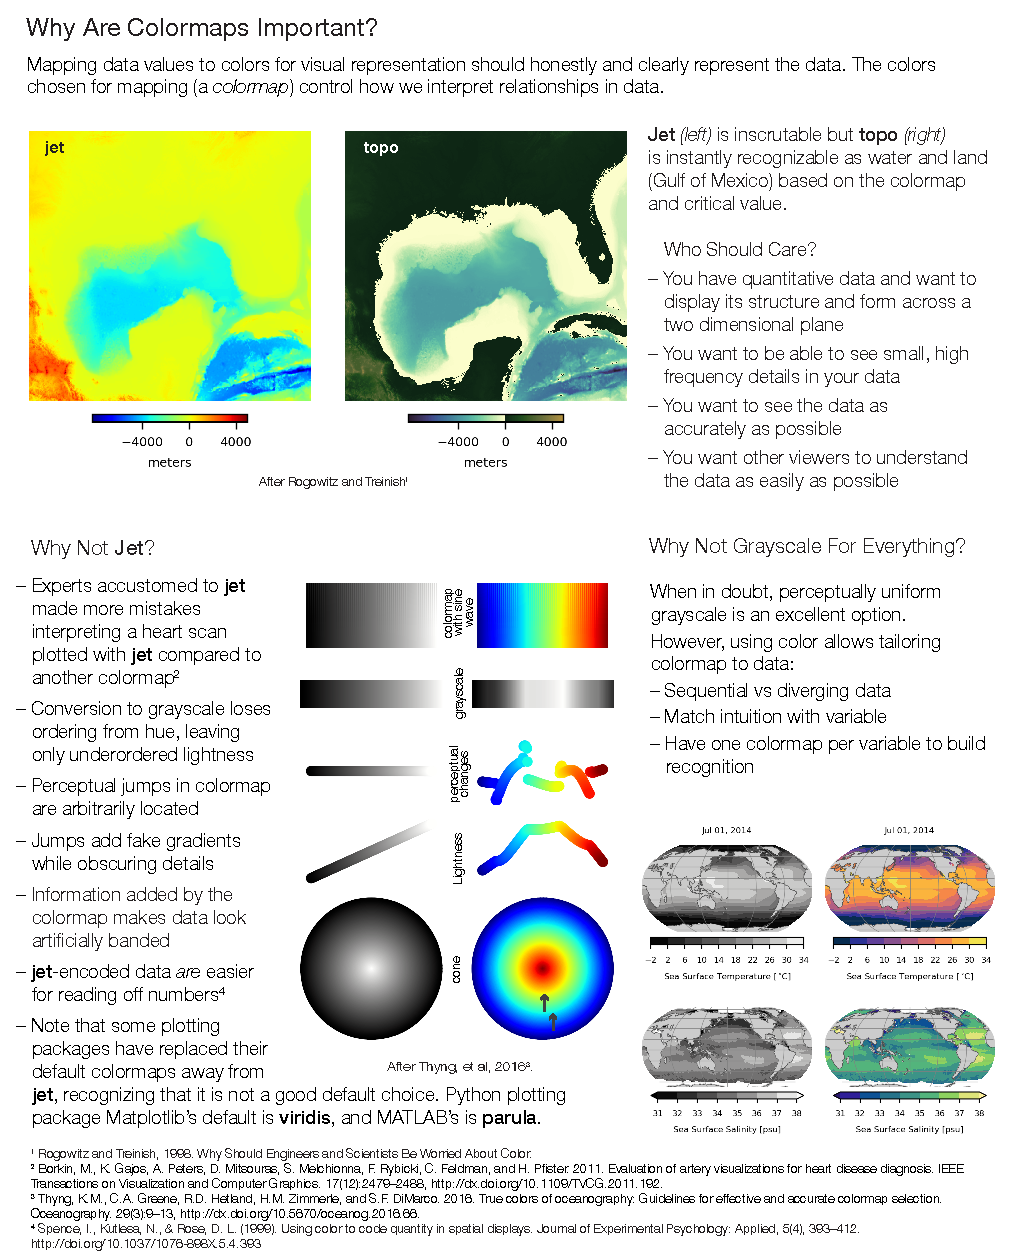
\includegraphics[width=\textwidth]{figures/illustrator/draft3/motivation.pdf}
	\caption{}
	\label{fig:motivation}
\end{figure*}

\nocite{treinish1998should}
\nocite{borkin2011evaluation}
\nocite{thyng2016true}



Color is represented by three dimensions, called a colorspace. All colorspaces approximate how humans see color and use different dimensions for this representation. If a colormap is created from a perceptually-uniform colorspace, it has the special property that any equal distance along the colormap is perceived by humans as approximately equal in magnitude of change (Fig.~\ref{fig:evaluation}). A consequence of not using a perceptually-uniform colormap is perceptual jumps across the colormap, which can be large. These perceptual jumps introduce fake gradients into the data representation as well as obscure detail. Another important finding from previous studies is that humans best understand the relative form of data when it is mapped by lightness rather than hue \citep{kovesi2015good}.


\begin{figure*}
	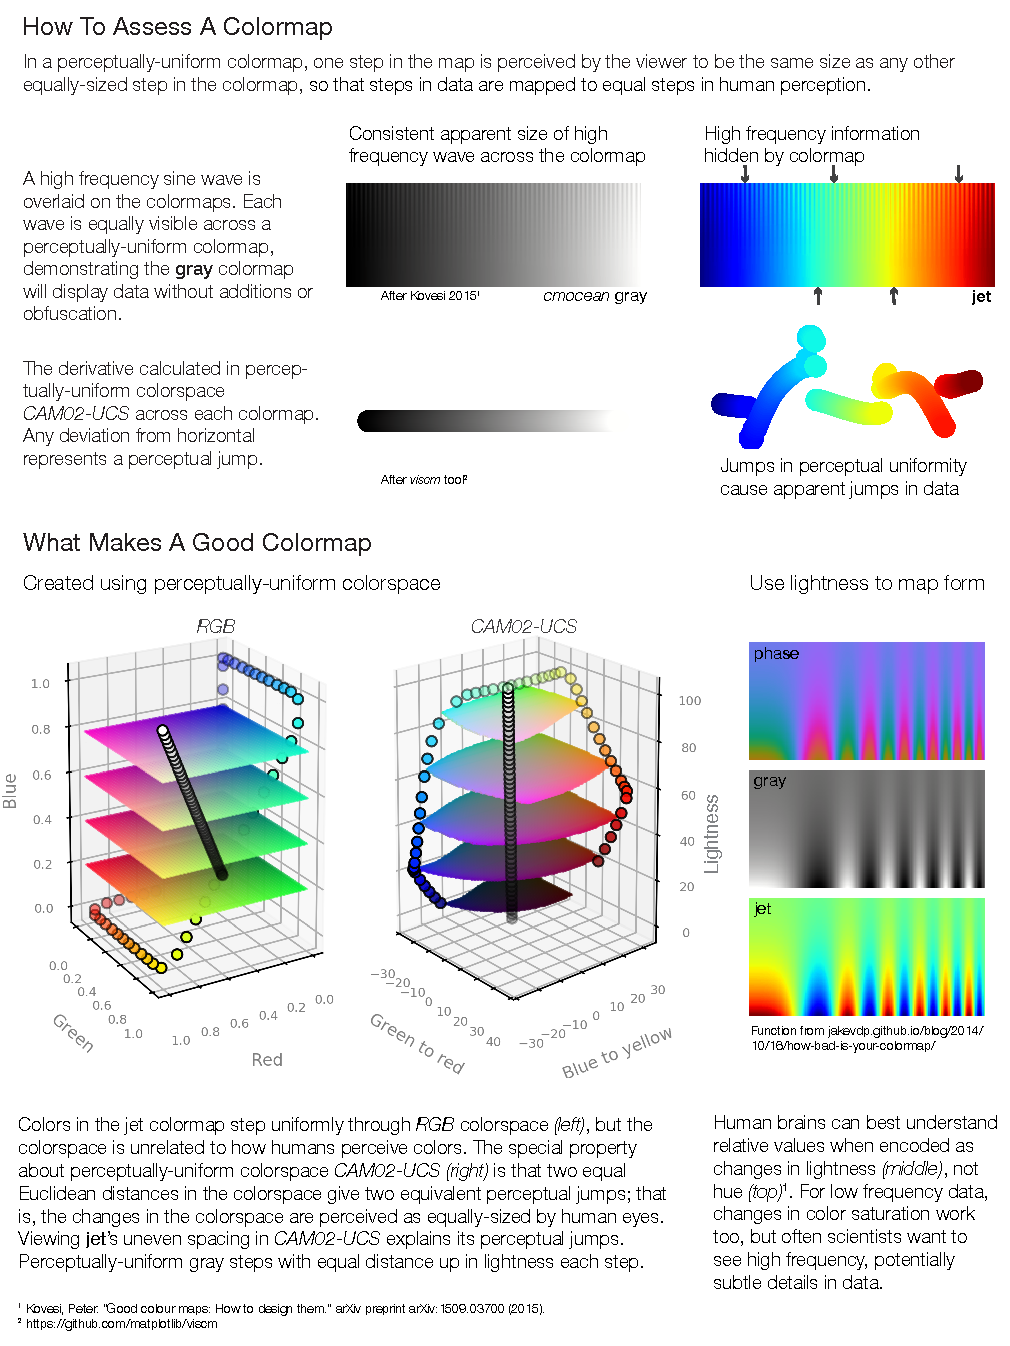
\includegraphics[width=\textwidth]{figures/illustrator/draft3/evaluation.pdf}
	\caption{}
	\label{fig:evaluation}
\end{figure*}
\nocite{kovesi2015good}
\nocite{viscm}



Colormaps for plotting relative data (rather than categorical data) can be generally grouped into 3 categories. First, sequential colormaps have monotonic lightness change and should be used to represent data that increases in size (such as chlorophyll, Fig.~\ref{fig:howtochoose}). Second, diverging colormaps have monotonic increase or decrease in lightness to a point, then change to monotonically decrease or increase. The utility of a diverging colormap is in representing data values relative to a critical point (for example, sea surface height relative to mean sea level). Third, cyclic colormaps should be used to represent data that cycles around a circle, like tidal phase. They should either not vary in lightness at all and cycle through hue only, or should cycle in both lightness and hue such that there is no major perceptual break in the colormap.

There are many considerations that should be taken into account when choosing the appropriate colormap for data presentation. For example, some form of color-blindness impacts about 7\% of Northern European, 4\% of Asian, and 3\% of African-descendent men \citep{sharpe1999opsin}. Avoiding colormaps that include both red and green, which look similar with the most common form of colorblindness, would be wise to invite a wider audience to the plot.


\begin{figure*}
	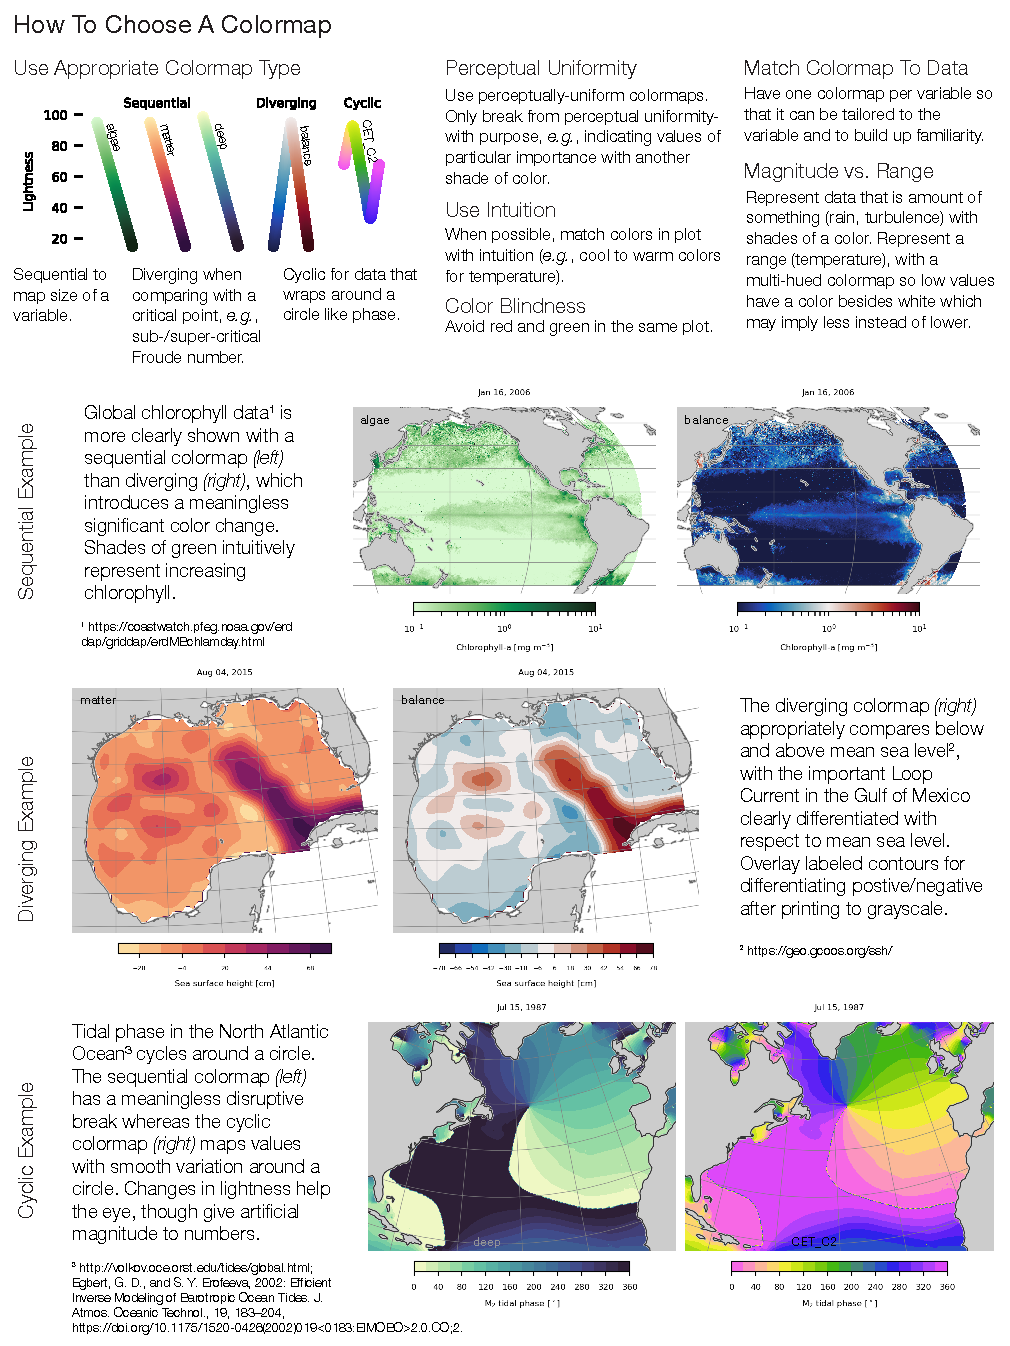
\includegraphics[width=\textwidth]{figures/illustrator/draft3/howtochoose.pdf}
	\caption{}
	\label{fig:howtochoose}
\end{figure*}
% Data sources
\nocite{chlor}
\nocite{ssh}
\nocite{egbert2002efficient}


A wide variety of reasonable, available colormaps are presented in Fig.~\ref{fig:allmaps}. Colormaps are plotted by the lightness as calculated in perceptually-uniform colorspace \textit{CAM02-UCS} in order to demonstrate this important property for making a colormap choice.

\begin{figure*}
	\includegraphics[width=\textwidth]{figures/illustrator/draft3/allmaps.pdf}
	\caption{}
	\label{fig:allmaps}
\end{figure*}
% colormaps
\nocite{matplotlib}
\nocite{nunez2018optimizing}
\nocite{cubehelix}
\nocite{twilight}
\nocite{matlab}
\nocite{mycarta}
\nocite{light2004end}
\nocite{brewer}
\nocite{crameri2018geodynamic}


\section{Conclusion}

Colormaps have fundamental control over interpretation of data, and thus should be given some attention. Background information based on human perception of color as well as some basic design advice has been presented to guide selections.



\bibliographystyle{IEEEtran}
\bibliography{./refs}

\bigskip

\textbf{Kristen Thyng} is an assistant research professor of oceanography at Texas A\&M University. Her research interests include coastal physics, numerical modeling, visualization, and data science. She received a Ph.D. in mechanical engineering from the University of Washington, USA. Contact her at kthyng@tamu.edu.



\end{document}
